\graphicspath{{figures/appendix/}}
\chapter{Test Journal: Potentiometer}\label{appendix:PotMeterTest}
\begin{table}[!h]
\begin{tabular}{l l}
\textbf{Test participants:} & Mathias  \\
\textbf{Date:}  & 20/04-2017
\end{tabular}
\end{table}

\section*{Purpose}
The purpose of the test is to find the angle which corresponds to the voltages of the potentiometers. This will be done for both the arm potentiometer and stick potentiometer.
\section*{Test equipment and components}
\begin{table}[htbp]
	\centering
	\caption{List of measurement equipment and components}\label{tab_appendix:PotMeterMaterial}
	\begin{tabularx}{\textwidth}{lXXXX}
		Name & Brand & Model & AAU-number \\ \toprule
		Multimeter	& Fluke & 37 & 08181 	\\ \rowcolor{lightGrey}
		Oscilloscope	& Agilent & 54621D & 33941 	\\
		Power supply	& Agilent & E3631A & 78577\\ 
		\rowcolor{lightGrey}	
		DC motor & Alsthom BBC & F9M2& 08339\\
		Potentiometer & Bourns & Linear 10 k$\Omega$\newline 0,5\% linearity&\\ 		\rowcolor{lightGrey}
		Potentiometer & Bourns & Linear 10 k$\Omega$\newline 1\% linearity&\\
		Protractor & & &\\ \rowcolor{lightGrey}
		Spirit level & & &
	\end{tabularx}
\end{table}
\section*{Setup}
Measurement setup is seen on \autoref{fig:DCSetup} \
\begin{figure} [htbp]
\hspace*{-3.7cm}  
\centering
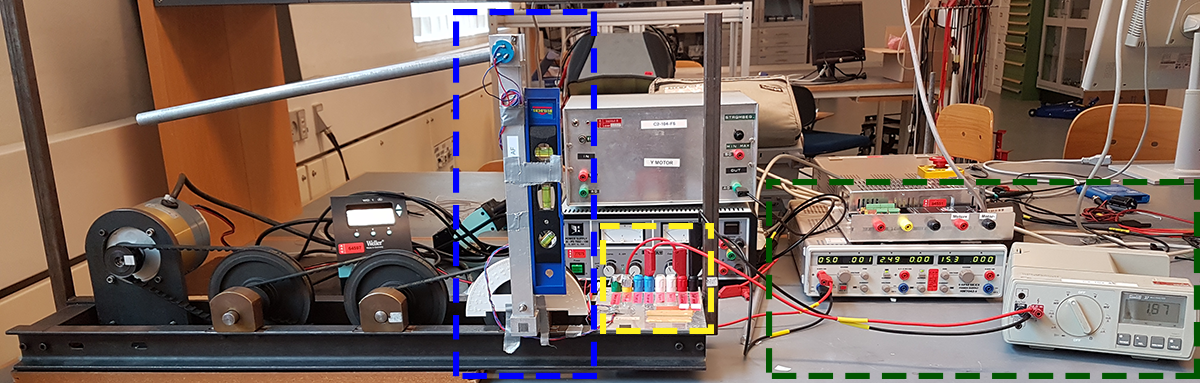
\includegraphics[width=0.95\paperwidth]{figures/appendix/Motor&GearTests/PotMeterSetup}
\caption{Measurement setup.}
\label{fig:DCSetup}
\end{figure}


\startexplain
\explain{\textbf{Blue box} contains the arm, with protractor and spirit level tool. The potentiometer is placed on the back of the opposite site of the arm axis.}{}
\explain{\textbf{Green box} contains the power supply and voltmeter.}{}
\explain{\textbf{Yellow box} contains the power inputs and sensor outputs.}{}
\stopexplain

\section*{Method}
The procedure for the test is as following:
\begin{enumerate}
\item Supply the sensor with 5 V and ground trough the input and output connection board in the yellow box. 
\item Attached the potentiometer of the arm to the voltmeter, the stick is not considered during measurement of the arm.
\item Use the spirit level to place the arm in vertical position which is the systems 0$^\circ$
\item Note the voltage.
\item Use the spirit level and protractor to place the arm in anti clockwise -45$^\circ$ from vertical.
\item Note the voltage, and repeat earlier with -90$^\circ$, +45$^\circ$ and +90$^\circ$ 
\item Place the arm in 0$^\circ$ and lock it.
\item Change the voltmeter to read the output from the stick potentiometer. 
\end{enumerate}
\section*{Raw data}
Voltages from each potentiometer is not expected to be the same. This is based on that the initial orientation of the potentiometers is not the same. 
\begin{table}[htbp]
\centering
\begin{tabular}{lll}
\hline
Position ($^\circ$) & Voltage Pot$_{arm}$ (V) & Voltage Pot$_{stick}$ (V) \\ \hline
-90$^\circ$         & 0,437 V                 & 1,200 V                   \\
-45$^\circ$         & 1,146 V                 & 1,89 V                   \\
0$^\circ$           & 1,860 V                 & 2,558 V                   \\
45$^\circ$          & 2,573 V                 & 3,23 V                   \\
90$^\circ$          & 3,270 V                 & 3,90 V                   
\end{tabular}
\caption{Angle position and corresponding voltage.}
\label{AngleTable}
\end{table}
\section*{Data processing}
The main objective to determine is outer limit and how much 1 V corresponds to in angle change. This can give the possibility to convert the analogue input on an Arduino back to the corresponding angle. 


It is shown that the linearity is acceptable and the proportional angle to voltage conversion is considered linear.
The conversion must be separated into two parts. This is done because the angle to voltage is different between the potentiometers.
To obtain i first order function the voltages and angles is plotted and approximated for both potentiometers.

\begin{figure}[htbp]
\hspace*{-3cm}  
\centering
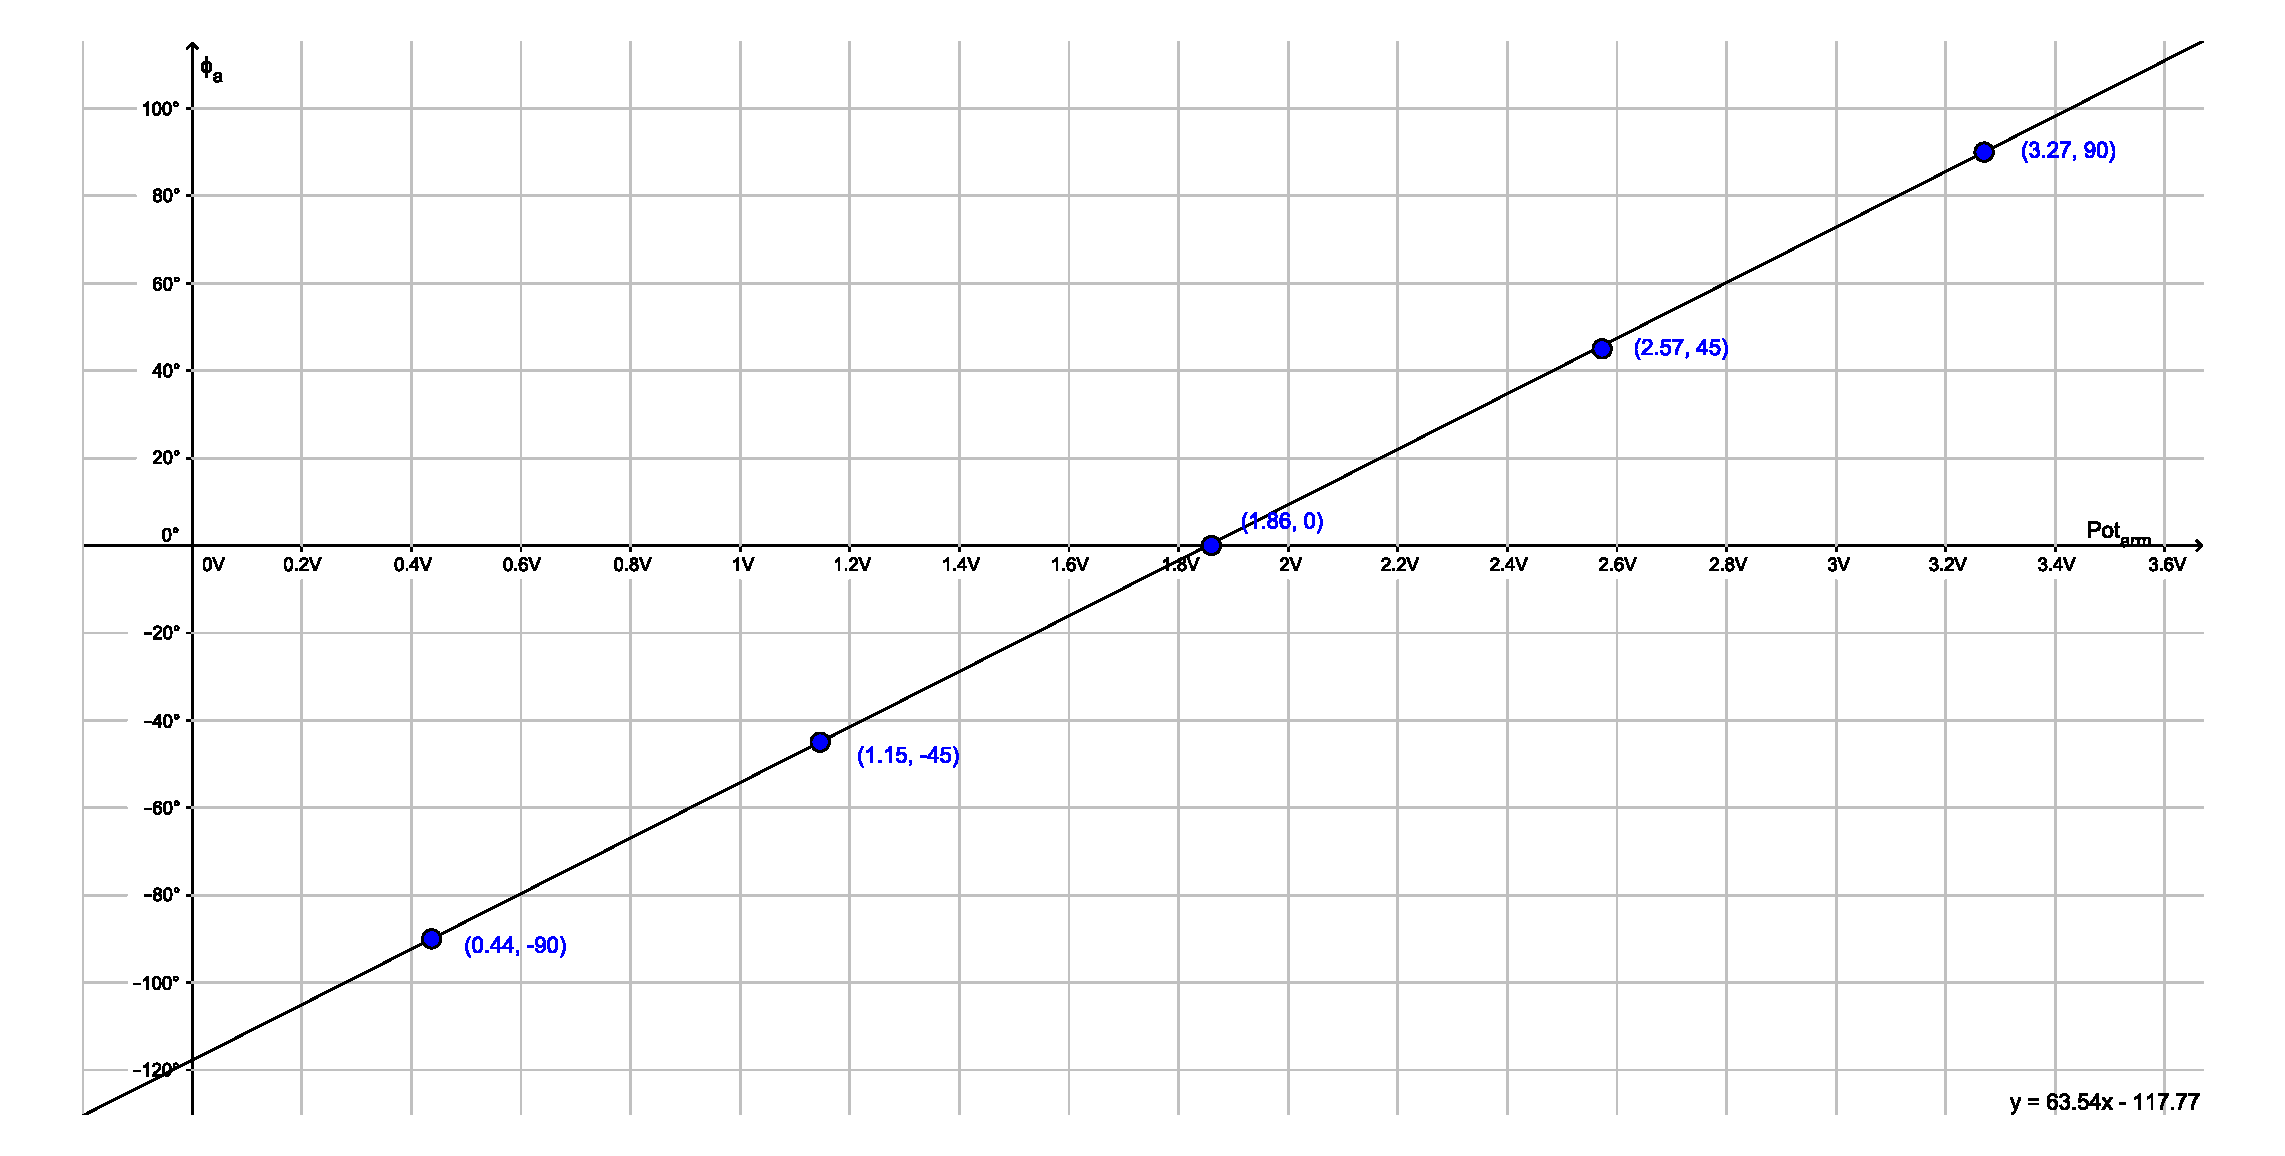
\includegraphics[width=0.95\paperwidth]{figures/appendix/PotentiometerPlot.pdf}
\caption{First order approximation of the arm potentiometer.}
\label{fig:PotentiometerPlot}
\end{figure}
\bigbreak

This approximation corresponds to a relation between the voltage to angle of the arm on figure \ref{fig:PotentiometerPlot}.
\begin{equation}
\theta_a\ =\ 63,64 \cdot \text{VPot}_{arm} - 117,77
\end{equation}
\newpage
The plot is repeated for the potentiometer on the stick.
\begin{figure}[htbp]  
\hspace*{-3cm}
\centering
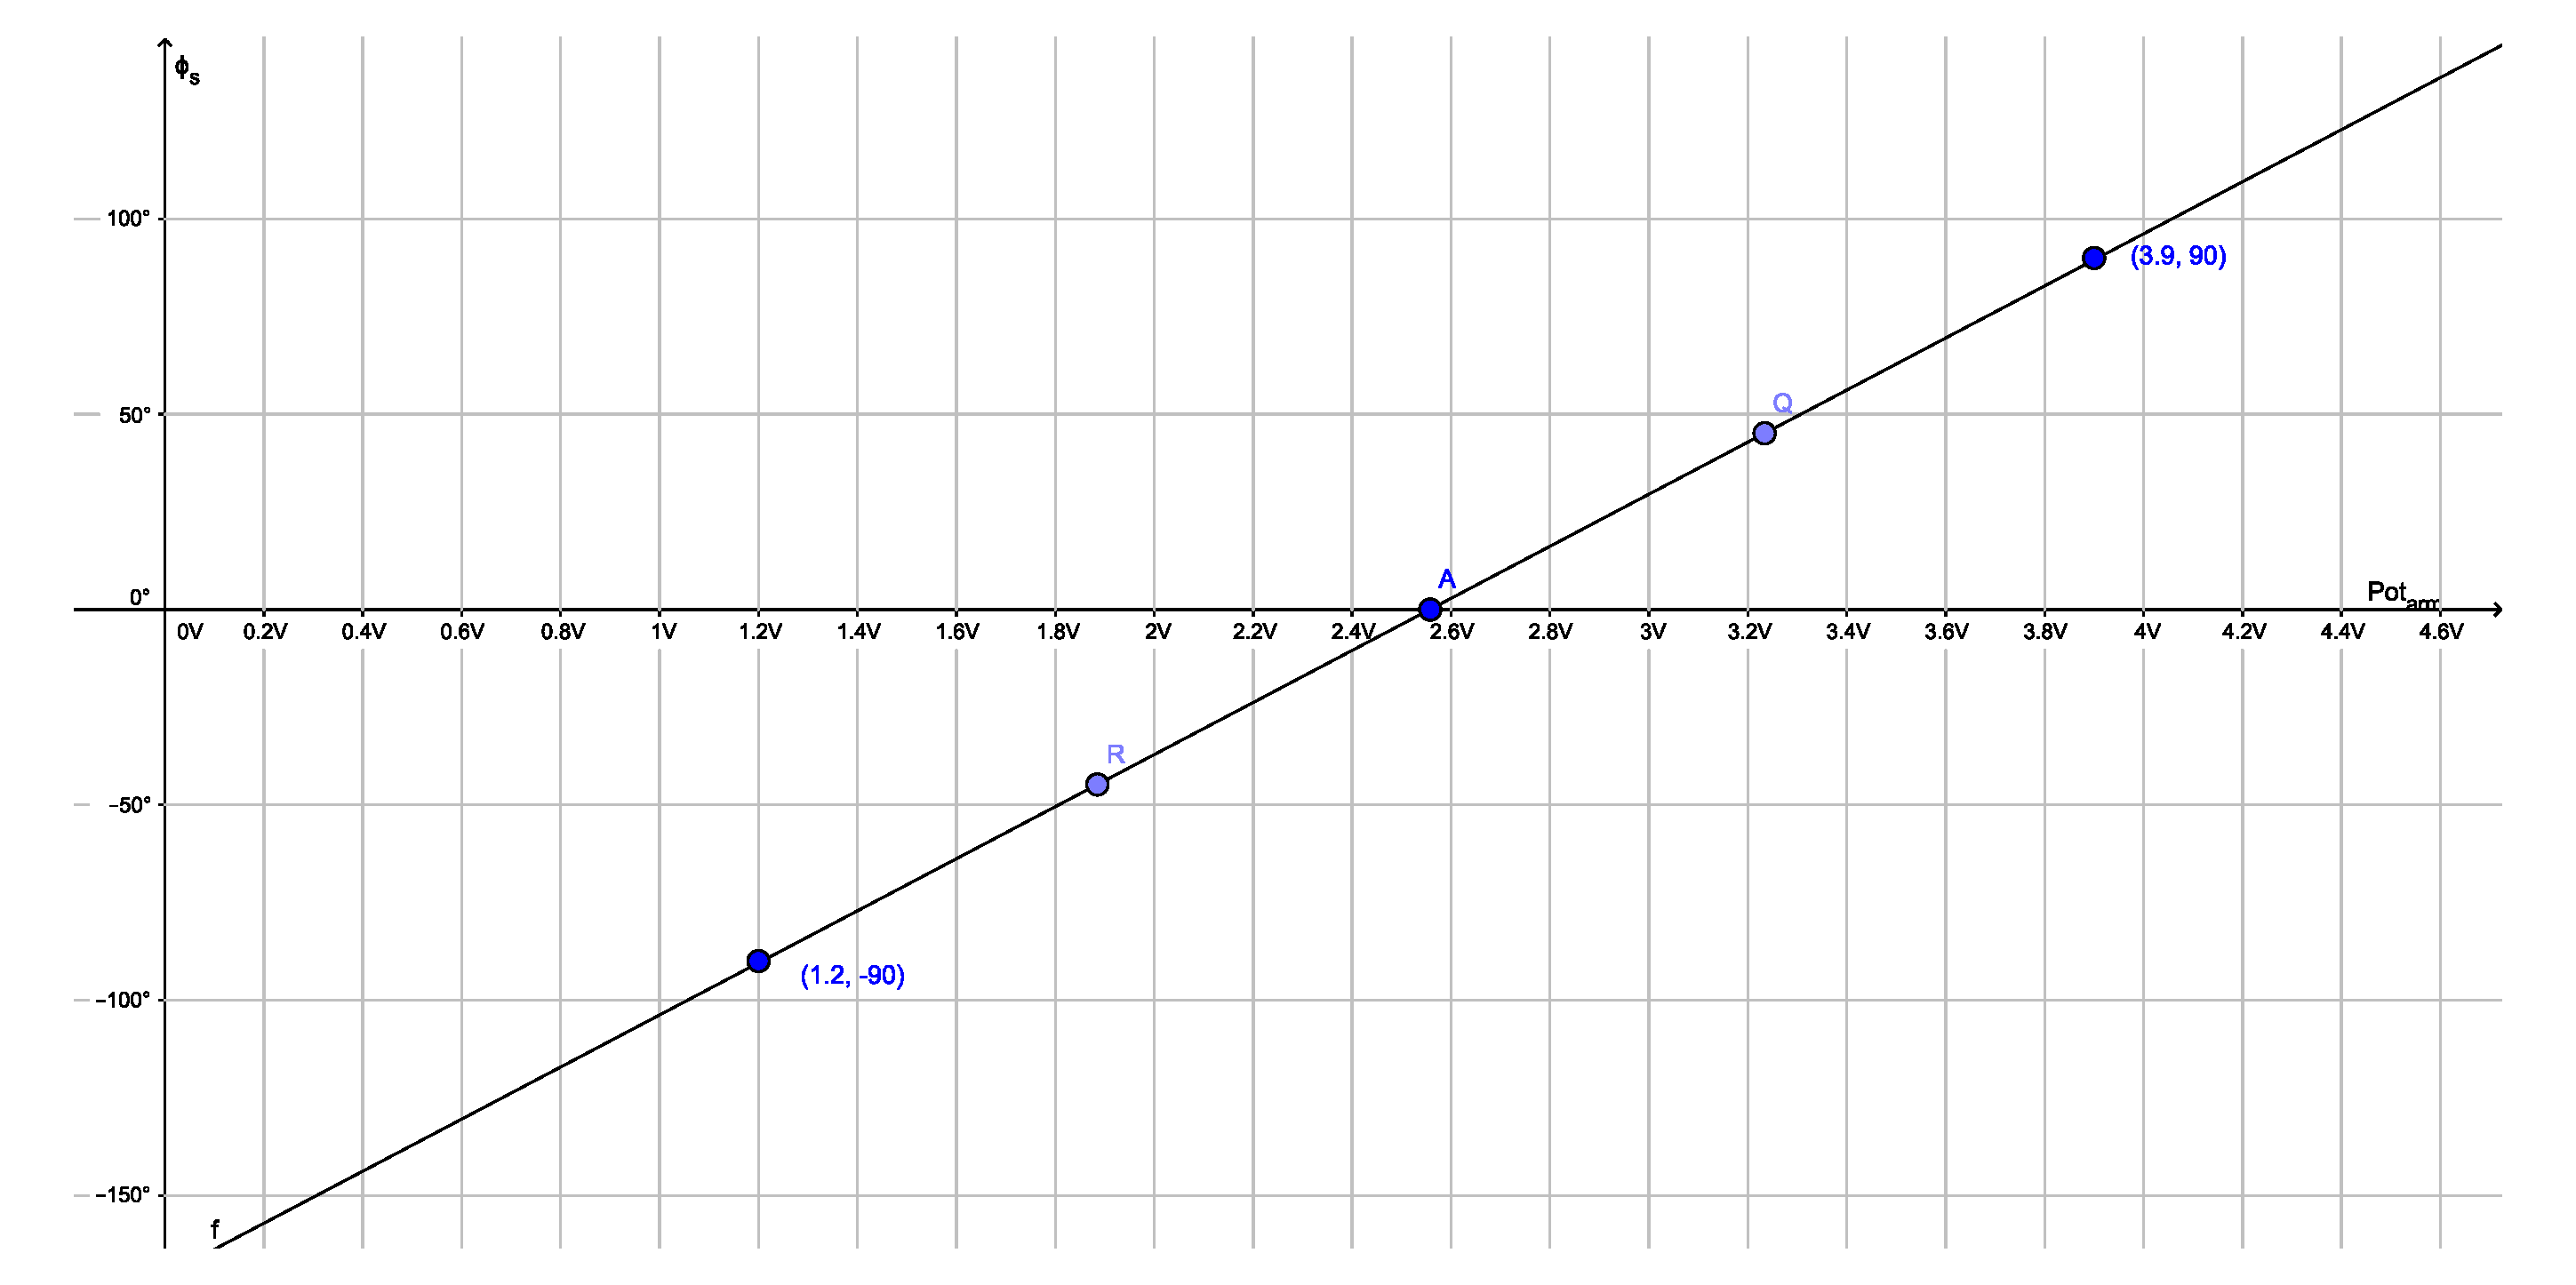
\includegraphics[width=0.95\paperwidth]{figures/appendix/PotentiometerPlotStick.pdf}
\caption{First order approximation of the stick potentiometer.}
\label{fig:PotentiometerPlotStick}
\end{figure}

This approximation that corresponds to a relation between the voltage to angle of the arm on figure \ref{fig:PotentiometerPlot}.
\begin{equation}
\theta_s\ =\ 66,66 \cdot \text{VPot}_{stick} - 170,46
\end{equation}

Sampling the sensor with an Arduino will be done trough reading the voltage on an input. The voltage will corresponds to an proportional analog value from 0-1023, where 0 V = 0 and 5 V = 1023. Translating the voltages into angles can give us the backwards conversion. Considering that the value can take 1024 values then:
\begin{equation}
\dfrac{1024\ \text{units}}{5\ \text{V}} = 204,8\ \text{units/V}
\end{equation}     
Considering that the precision of the measurements and using an Arduino, all values would be rounded to the nearest integer.
The linear approximations might be calibrated during implementation to minimize offsets.
Further implementation is processed cf. section \ref{section:PotmeterImplementation}.

\section*{Conclusion}
The tested concludes that it is possible to convert the voltage to values that can be used with an Arduino. The test also concludes that is a use able linearity of both potentiometers when during conversions. Though the precision of the measurements shall be considered even though the measurements had similarities. 

